\documentclass{ximera}

%\usepackage{todonotes}

\newcommand{\todo}{}

\usepackage{tkz-euclide}
\tikzset{>=stealth} %% cool arrow head
\tikzset{shorten <>/.style={ shorten >=#1, shorten <=#1 } } %% allows shorter vectors

\usepackage{tkz-tab}  %% sign charts
\usetikzlibrary{decorations.pathreplacing} 

\usetikzlibrary{backgrounds} %% for boxes around graphs
\usetikzlibrary{shapes,positioning}  %% Clouds and stars
\usetikzlibrary{matrix} %% for matrix
\usepgfplotslibrary{polar} %% for polar plots
\usetkzobj{all}
\usepackage[makeroom]{cancel} %% for strike outs
%\usepackage{mathtools} %% for pretty underbrace % Breaks Ximera
\usepackage{multicol}

\usepackage{polynom}



\usepackage[many]{tcolorbox}  %% for titled boxes
\newtcolorbox{xbox}[1]{%
    tikznode boxed title,
    enhanced,
    arc=0mm,
    interior style={white},
    attach boxed title to top center= {yshift=-\tcboxedtitleheight/2},
    fonttitle=\bfseries,
    colbacktitle=white,coltitle=black,
    boxed title style={size=normal,colframe=white,boxrule=0pt},
    title={#1}}


\usepackage{array}
\setlength{\extrarowheight}{+.1cm}   
\newdimen\digitwidth
\settowidth\digitwidth{9}
\def\divrule#1#2{
\noalign{\moveright#1\digitwidth
\vbox{\hrule width#2\digitwidth}}}





\newcommand{\RR}{\mathbb R}
\newcommand{\R}{\mathbb R}
\newcommand{\N}{\mathbb N}
\newcommand{\Z}{\mathbb Z}

%\renewcommand{\d}{\,d\!}
\renewcommand{\d}{\mathop{}\!d}
\newcommand{\dd}[2][]{\frac{\d #1}{\d #2}}
\newcommand{\pp}[2][]{\frac{\partial #1}{\partial #2}}
\renewcommand{\l}{\ell}
\newcommand{\ddx}{\frac{d}{\d x}}
\newcommand{\ddt}{\frac{d}{\d t}}

\newcommand{\zeroOverZero}{\ensuremath{\boldsymbol{\tfrac{0}{0}}}}
\newcommand{\inftyOverInfty}{\ensuremath{\boldsymbol{\tfrac{\infty}{\infty}}}}
\newcommand{\zeroOverInfty}{\ensuremath{\boldsymbol{\tfrac{0}{\infty}}}}
\newcommand{\zeroTimesInfty}{\ensuremath{\small\boldsymbol{0\cdot \infty}}}
\newcommand{\inftyMinusInfty}{\ensuremath{\small\boldsymbol{\infty - \infty}}}
\newcommand{\oneToInfty}{\ensuremath{\boldsymbol{1^\infty}}}
\newcommand{\zeroToZero}{\ensuremath{\boldsymbol{0^0}}}
\newcommand{\inftyToZero}{\ensuremath{\boldsymbol{\infty^0}}}



\newcommand{\numOverZero}{\ensuremath{\boldsymbol{\tfrac{\#}{0}}}}
\newcommand{\dfn}{\textbf}
%\newcommand{\unit}{\,\mathrm}
\newcommand{\unit}{\mathop{}\!\mathrm}
\newcommand{\eval}[1]{\bigg[ #1 \bigg]}
\newcommand{\seq}[1]{\left( #1 \right)}
\renewcommand{\epsilon}{\varepsilon}
\renewcommand{\iff}{\Leftrightarrow}

\DeclareMathOperator{\arccot}{arccot}
\DeclareMathOperator{\arcsec}{arcsec}
\DeclareMathOperator{\arccsc}{arccsc}
\DeclareMathOperator{\si}{Si}
\DeclareMathOperator{\proj}{proj}
\DeclareMathOperator{\scal}{scal}


\newcommand{\tightoverset}[2]{% for arrow vec
  \mathop{#2}\limits^{\vbox to -.5ex{\kern-0.75ex\hbox{$#1$}\vss}}}
\newcommand{\arrowvec}[1]{\tightoverset{\scriptstyle\rightharpoonup}{#1}}
\renewcommand{\vec}{\mathbf}
\newcommand{\veci}{\vec{i}}
\newcommand{\vecj}{\vec{j}}
\newcommand{\veck}{\vec{k}}
\newcommand{\vecl}{\boldsymbol{\l}}

\newcommand{\dotp}{\bullet}
\newcommand{\cross}{\boldsymbol\times}
\newcommand{\grad}{\boldsymbol\nabla}
\newcommand{\divergence}{\grad\dotp}
\newcommand{\curl}{\grad\cross}
%\DeclareMathOperator{\divergence}{divergence}
%\DeclareMathOperator{\curl}[1]{\grad\cross #1}


\colorlet{textColor}{black} 
\colorlet{background}{white}
\colorlet{penColor}{blue!50!black} % Color of a curve in a plot
\colorlet{penColor2}{red!50!black}% Color of a curve in a plot
\colorlet{penColor3}{red!50!blue} % Color of a curve in a plot
\colorlet{penColor4}{green!50!black} % Color of a curve in a plot
\colorlet{penColor5}{orange!80!black} % Color of a curve in a plot
\colorlet{fill1}{penColor!20} % Color of fill in a plot
\colorlet{fill2}{penColor2!20} % Color of fill in a plot
\colorlet{fillp}{fill1} % Color of positive area
\colorlet{filln}{penColor2!20} % Color of negative area
\colorlet{fill3}{penColor3!20} % Fill
\colorlet{fill4}{penColor4!20} % Fill
\colorlet{fill5}{penColor5!20} % Fill
\colorlet{gridColor}{gray!50} % Color of grid in a plot

\newcommand{\surfaceColor}{violet}
\newcommand{\surfaceColorTwo}{redyellow}
\newcommand{\sliceColor}{greenyellow}




\pgfmathdeclarefunction{gauss}{2}{% gives gaussian
  \pgfmathparse{1/(#2*sqrt(2*pi))*exp(-((x-#1)^2)/(2*#2^2))}%
}


%%%%%%%%%%%%%
%% Vectors
%%%%%%%%%%%%%

%% Simple horiz vectors
\renewcommand{\vector}[1]{\left\langle #1\right\rangle}


%% %% Complex Horiz Vectors with angle brackets
%% \makeatletter
%% \renewcommand{\vector}[2][ , ]{\left\langle%
%%   \def\nextitem{\def\nextitem{#1}}%
%%   \@for \el:=#2\do{\nextitem\el}\right\rangle%
%% }
%% \makeatother

%% %% Vertical Vectors
%% \def\vector#1{\begin{bmatrix}\vecListA#1,,\end{bmatrix}}
%% \def\vecListA#1,{\if,#1,\else #1\cr \expandafter \vecListA \fi}

%%%%%%%%%%%%%
%% End of vectors
%%%%%%%%%%%%%

%\newcommand{\fullwidth}{}
%\newcommand{\normalwidth}{}



%% makes a snazzy t-chart for evaluating functions
%\newenvironment{tchart}{\rowcolors{2}{}{background!90!textColor}\array}{\endarray}

%%This is to help with formatting on future title pages.
\newenvironment{sectionOutcomes}{}{} 



%% Flowchart stuff
%\tikzstyle{startstop} = [rectangle, rounded corners, minimum width=3cm, minimum height=1cm,text centered, draw=black]
%\tikzstyle{question} = [rectangle, minimum width=3cm, minimum height=1cm, text centered, draw=black]
%\tikzstyle{decision} = [trapezium, trapezium left angle=70, trapezium right angle=110, minimum width=3cm, minimum height=1cm, text centered, draw=black]
%\tikzstyle{question} = [rectangle, rounded corners, minimum width=3cm, minimum height=1cm,text centered, draw=black]
%\tikzstyle{process} = [rectangle, minimum width=3cm, minimum height=1cm, text centered, draw=black]
%\tikzstyle{decision} = [trapezium, trapezium left angle=70, trapezium right angle=110, minimum width=3cm, minimum height=1cm, text centered, draw=black]


\outcome{Solve linear inequalities.}
\outcome{Solve nonlinear inequalities using a sign chart.}

\title[Dig-In:]{Inequalities}
\begin{document}
\begin{abstract}
  We discuss inequalities.
\end{abstract}
\maketitle

Devyn asked what score was needed on the third exam to have an average of 82.  This gave us the equation $\displaystyle \dfrac{74 + 84 + x}{3} = 82$.  
The solutions only tell us what will give an average \emph{exactly} 82.  It may have been more advantageous to ask what score was needed to have an
average of at least 82, yielding not an equation, but an \emph{inequality}, $\displaystyle \dfrac{74+84+x}{3} \geq 82$.

As with equations, there are various types of inequalities.  

A \emph{linear inequality in $x$} is an inequality which is equivalent to  $ax + b >0$, $ax + b \geq 0$, $ax+b < 0$, or $ax + b \leq 0$.
We solve the inequality in much the same manner as with a linear equation.  The main differences come from changing the direction of the inequality when multiplying/dividing
by a negative quantity and expressing our answers in interval notation.

\begin{example}
 	Solve the inequality $\displaystyle \dfrac{2x}{3}-4 < 3\left( 2-x \right)$.
	\begin{explanation}
    		As with equations, we'll start by simplifying and combining like terms.
		\begin{align*}
			\dfrac{2x}{3} -4 &< 3\left( 2-x \right)\\
			\dfrac{2x}{3} - 4 &< 6 - 3x\\
			\dfrac{2x}{3}+3x &< 6 + 4\\
			\dfrac{11}{3} x &< 10\\
			x &< \dfrac{30}{11}
		\end{align*}
		All $x$ less than $\frac{30}{11}$ satisfy the inequality.
		
		The solution is $\left( -\infty , \dfrac{30}{11} \right)$.
	\end{explanation}
\end{example}

Nonlinear inequalities are more complicated.  To solve them, we will use a tool called a \emph{sign chart}.
The process requires us to move all the nonzero terms of the inequality to one side, and factor.
\begin{example}
	Solve the inequality \[ \dfrac{x^3 \left(2x-5\right)^2}{x+1} > 0.\]

	\begin{explanation}
		Since the right-hand side is zero, we are really asking where the left-hand side will be positive.  The only way
		a nice formula like the left-hand side can switch from positive to negative, or vice-versa, is if it is either zero
		or undefined at the point where it changes.

		Notice where the left-hand side would be either zero or undefined.  Those occur at $x = -1, 0, \frac{5}{2}$.  
		We'll use those points to split the number line into four regions. Inside each of those regions, our factors are either
		always positive or always negative.
		
		\begin{tikzpicture} 
			\tkzTabInit[lgt=2,espcl=1] 
				{$x$         /1, 
				$x^3$   /1, 
				$\left(2x-5\right)^2$  /1,
				$x+1$       /1}% 
				{  , $-1$ , $0$ ,$\dfrac{5}{2}$,  }% 
			\tkzTabLine{ , - , d , - , t , + , t , + ,}
			\tkzTabLine{ , + , d , + , t , + , t , + ,}
			\tkzTabLine{ , - , d , + , t , + , t , +, }
		\end{tikzpicture} 
		
		For $x < -1$, we find $x^3 < 0$, $(2x-5)^2 > 0$, and $x+1 < 0$.  Together, that means the left-hand side of our inequality has the form 
		$\displaystyle \dfrac{ \textrm{negative} \cdot \textrm{positive}}{\textrm{negative}}$.  It is, therefore, positive in that region, and makes up
		part of our solution.  We cannot include the endpoint $x=-1$ in the solution, as the fraction is undefined there.
		
		In the same way, we see that in the intervals $\left( 0, \frac{5}{2} \right)$ and $\left( \frac{5}{2}, 0\right)$, the left-hand side of the inequality is also positive.
		Notice that the inequality is NOT satisfied at $x=\frac{5}{2}$, where the left-hand side equals zero.  
		
		The solution is $\left( -\infty, -1 \right) \cup \left( 0, \frac{5}{2} \right) \cup \left( \frac{5}{2}, \infty \right)$.
	\end{explanation}
\end{example}


\begin{example}
	Solve the inequality \[ \dfrac{2x}{x-1} \leq \dfrac{5-x}{x-1}. \] 

	\begin{explanation}
		Let's start by moving all the terms to one side of the inequality.
		\begin{align*}
			\dfrac{2x}{x-1} &\leq \dfrac{5-x}{x-1}\\
			\dfrac{2x}{x-1} - \dfrac{5-x}{x-1} &\leq 0\\
			\dfrac{3x - 5}{x-1} &\leq 0
		\end{align*}
		\begin{tikzpicture} 
			\tkzTabInit[lgt=2,espcl=1] 
				{$x$         /1, 
				$3x-5$   /1, 
				$x-1$       /1}% 
				{  , $1$ , $\dfrac{5}{3}$,  }% 
			\tkzTabLine{ , - , d , - , t , + ,}
			\tkzTabLine{ , - , d , + , t , + ,}
		\end{tikzpicture} 
		The solution is $\displaystyle \left( 1, \dfrac{5}{3} \right]$.
	\end{explanation}
\end{example}

\begin{problem}
	Find the solution of the inequality \[ \dfrac{x}{x-4} \geq \dfrac{2x-1}{x-4}. \]
	\begin{multipleChoice}
		\choice[correct]{$\left[1, 4\right)$}
		\choice{$\left(-\infty, 1\right] \bigcup \left(4, \infty\right)$}
		\choice{$\left(1, 4\right)$}
		\choice{$\left(-\infty, 1\right) \bigcup \left(4, \infty\right)$}
		\choice{None of the above}
	\end{multipleChoice}
\end{problem}














\end{document}
